\documentclass{article}

\usepackage{a4wide}
\usepackage[utf8]{inputenc}
\usepackage[T1]{fontenc}
\usepackage[french]{babel}
\usepackage[babel=true]{csquotes} % guillemets français
\usepackage{graphicx}
\graphicspath{{Images/}}
\usepackage{color}
\usepackage{hyperref}
\hypersetup{colorlinks,linkcolor=,urlcolor=blue}

\usepackage{amsmath}
\usepackage{amssymb}


\title{Développement pour mobiles - Space Dynamics}
\author{Jean-Emile PELLIER, M1 informatique}
\date{\today}

\begin{document}

\maketitle % pour écrire le titre


%% Le résumé:
\begin{abstract}
  Space Dynamics est un jeu vidéo pour mobiles qui consiste à déplacer des balles à travers la galaxie afin qu’elles puissent atteindre leur destination le plus rapidement possible en évitant différents obstacles.
  
  Ce jeu de stratégie au gameplay volontairement simpliste s’est finalement révélé particulièrement complexe au cours de sa conception. En particulier, le choix d’utiliser des cercles pour tous les objets visibles aurait dû simplifier la conception mais il a fallu que ceux-ci la compliquent en devenant des ellipses du point de vue du mécanisme de détection des collisions.

  Dans ce document, nous allons étudier les fonctionnalités et l’implémentation de ce jeu.

\end{abstract}



\section*{Introduction}
Space Dynamics est un jeu vidéo conçu spécifiquement dans le cadre de ce projet. Il a été pensé pour être aussi simple que possible afin d’éviter de s’éterniser sur des mécanismes de jeu excessivement complexes au profit d’une utilisation plus poussée du potentiel matériel de l’appareil mobile.

Le jeu consiste à déplacer des balles colorées via l’inclinaison de l’appareil mobile jusqu’à leur destination de même couleur en allant le plus vite possible. En effet, un temps est affiché au-dessus de la partie courante, il va correspondre au score associé à la partie dès lors qu’elle sera terminée.

Plusieurs stratégies permettent de terminer une partie mais certaines d'entre elles sont plus rapides à mettre en oeuvre que d'autres, elles seront à privilégier dans la perspective d'obtenir un bon score. 

Le contexte global se déroule dans l’espace, l’objectif étant de se servir de la richesse des comportements des objets célestes pour bâtir un univers très dynamique d’où le nom du jeu.

L’ambiance générale se veut apaisante, elle est renforcée par une musique d’arrière-plan relaxante.

Dans cette version on ne va considérer que 4 entités distinctes :
\begin{itemize}
\item les balles jouables : contrôlables par le joueur via l’inclinaison de son appareil mobile
\item les cercles de destination : permettant de terminer un niveau de jeu par la capture des balles
\item les trous noirs : ramenant les balles à leur position initiale pour ralentir le joueur
\item les trous blancs : repoussant les balles au loin pour les éloigner de leur objectif.
\end{itemize}

Les balles jouables ne peuvent pas sortir de l’écran.
\bigbreak
Comment ce jeu vidéo mobile a-t-il été implémenté ?
\bigbreak
Etudions en détails les fonctionnalités et l’implémentation de ce jeu.



\section{Description générale de l'application}

\subsection{Menu principal}
\begin{center}
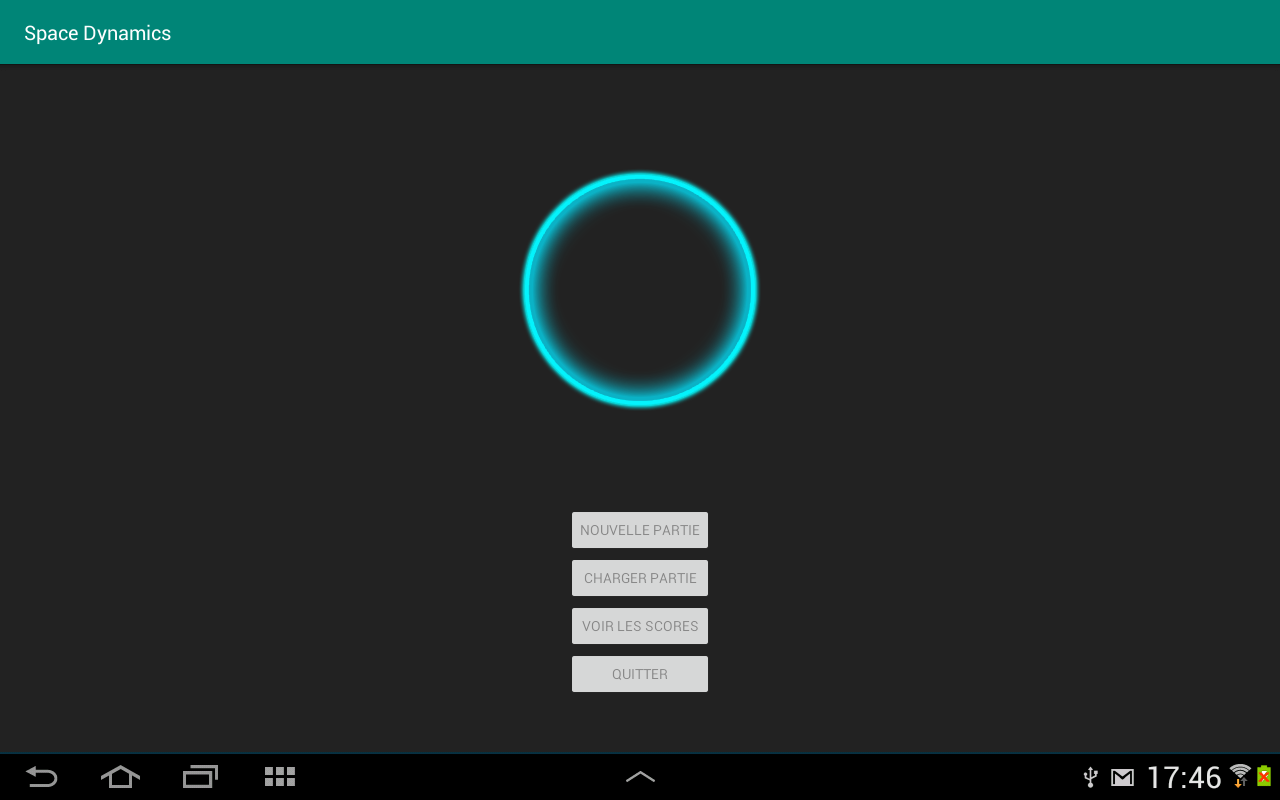
\includegraphics[scale=0.25]{MainMenuActivity.png}
\end{center}
Le menu principal offre au joueur la possibilité de :
\begin{itemize}
\item démarrer une nouvelle partie
\item charger une partie enregistrée
\item consulter la liste des scores enregistrés
\item quitter l'application
\end{itemize}

\subsection{Interface de jeu}
\begin{center}
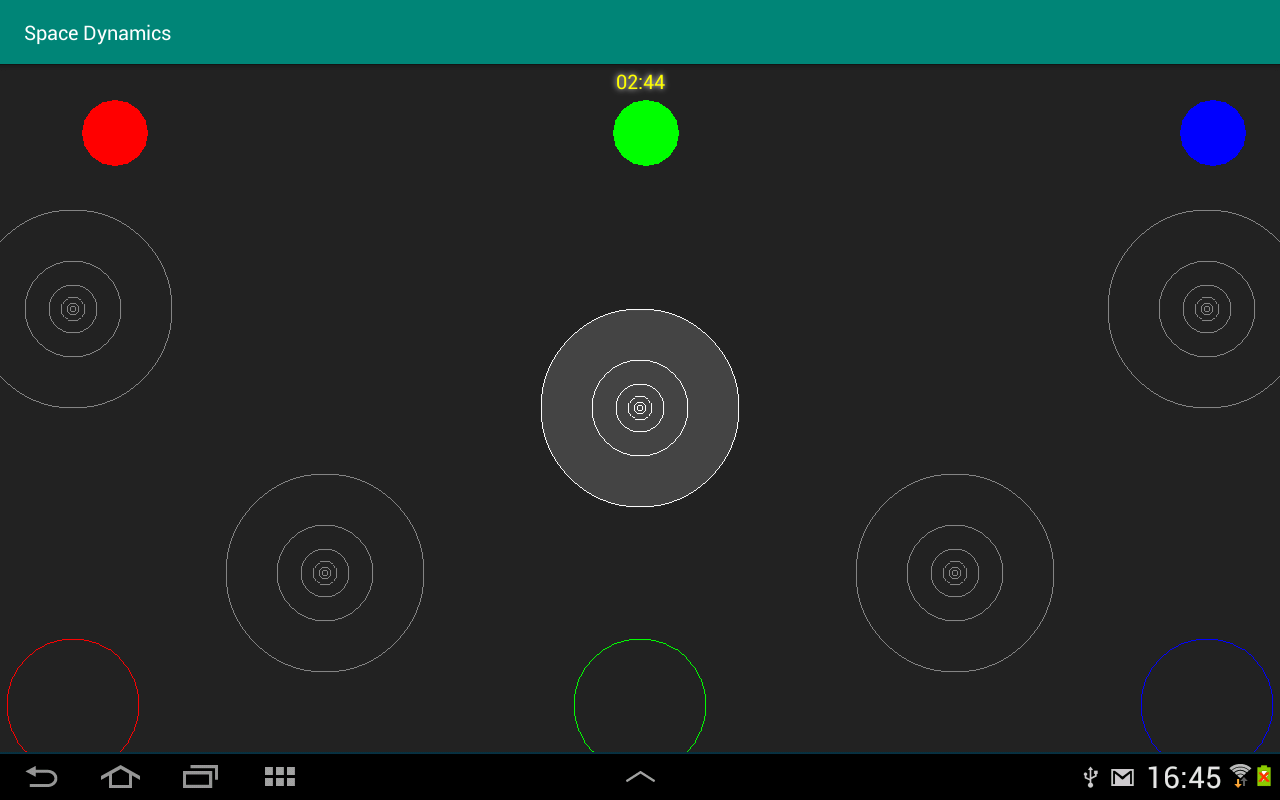
\includegraphics[scale=0.25]{PlayGameActivity.png}
\end{center}
L'interface de jeu propose de :
\begin{itemize}
\item jouer à Space Dynamics
\item déplacer les balles selon l’inclinaison de l’appareil mobile
\item faire une pause via un double tap
\end{itemize}
Dans cette capture d’écran on peut voir 3 balles jouables l’une rouge, une autre verte et une dernière bleue en haut de l’écran, accompagnées de leur cercles de destination en bas de l'écran. Quant aux cercles concentriques foncés et clairs, ils matérialisent respectivement les trous noirs et les trous blancs.

\subsection{Menu pause}
\begin{center}
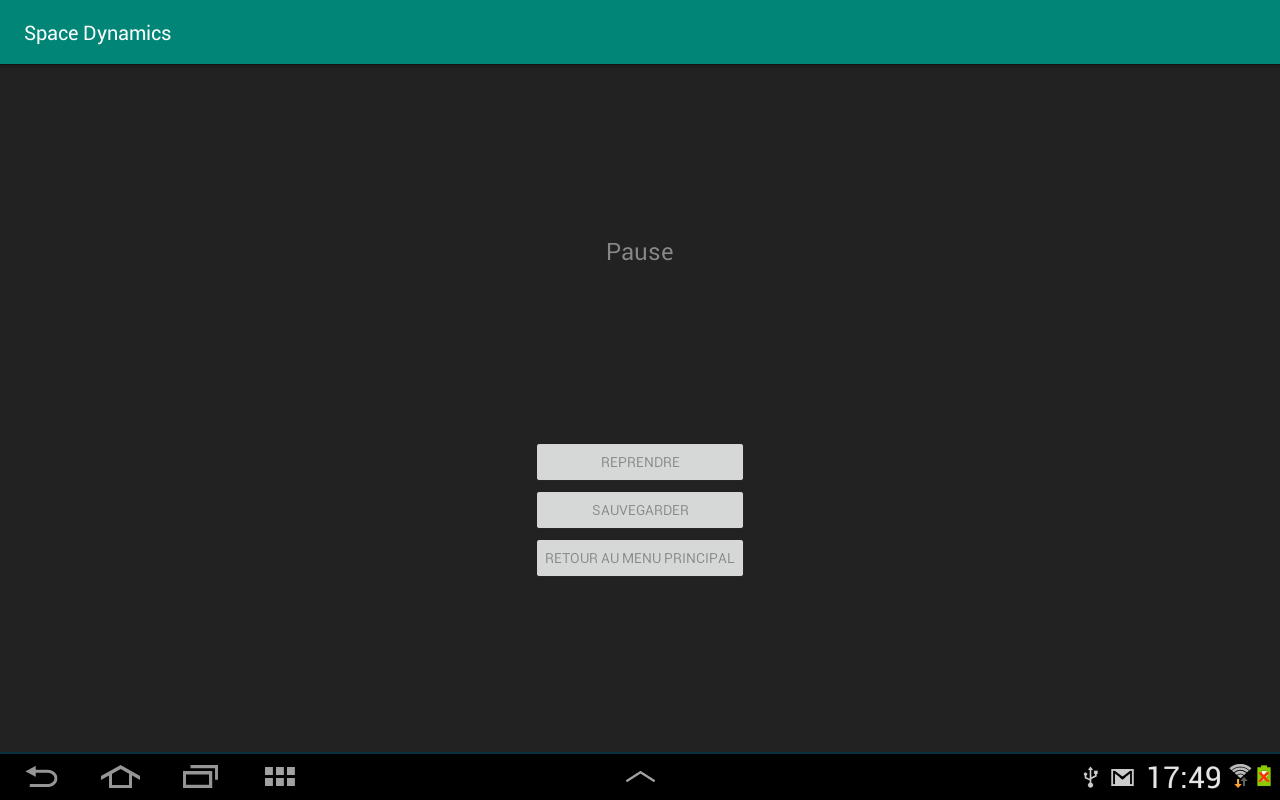
\includegraphics[scale=0.25]{PauseActivity.png}
\end{center}
Le menu pause propose au joueur de : 
\begin{itemize}
\item reprendre sa partie
\item sauvegarder l'état actuel de sa partie
\item retourner au menu principal
\end{itemize}

\subsection{Menu sauvegarder}
\begin{center}
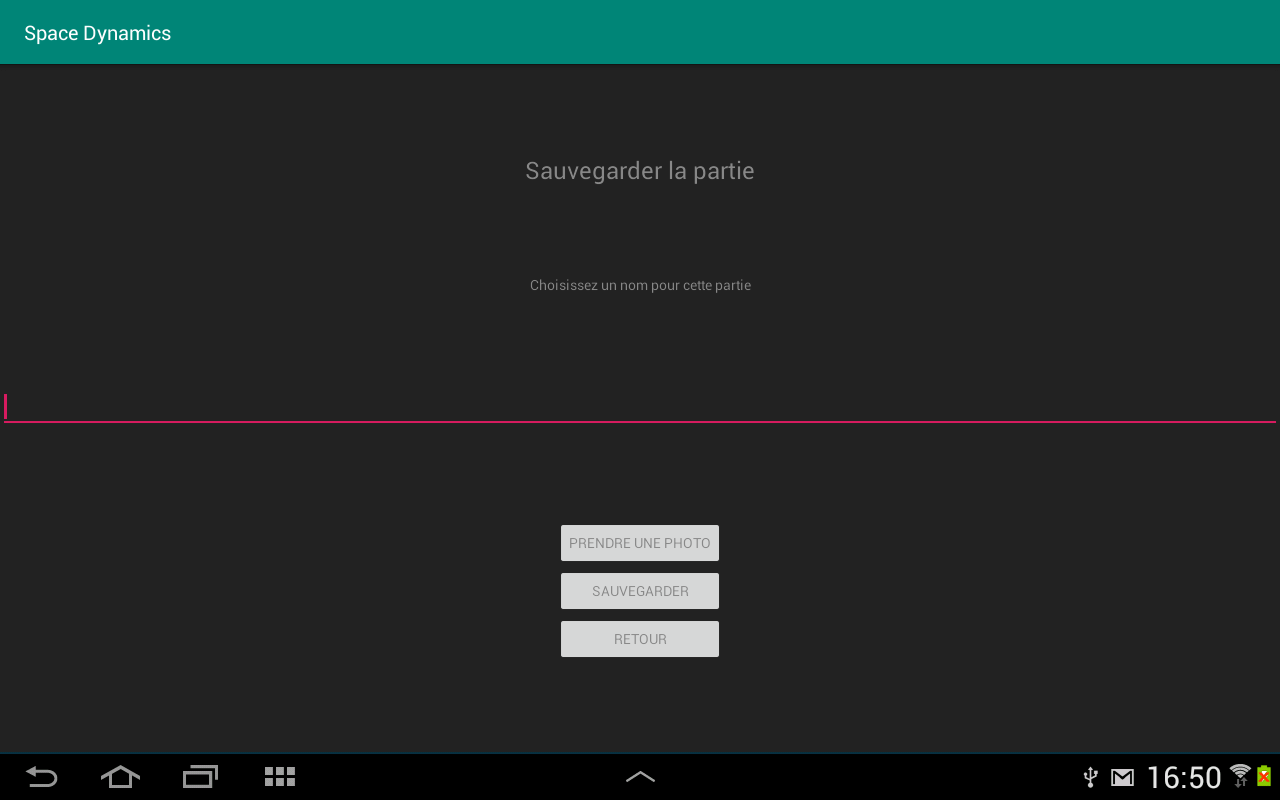
\includegraphics[scale=0.25]{SaveGameActivity.png}
\end{center}
Le menu de sauvegarde propose de :
\begin{itemize}
\item nommer la partie en cours
\item prendre une photo pour l’associer à la partie
\item sauvegarder la partie en cours
\item retourner au menu pause
\end{itemize}

\subsection{Menu caméra}
\begin{center}
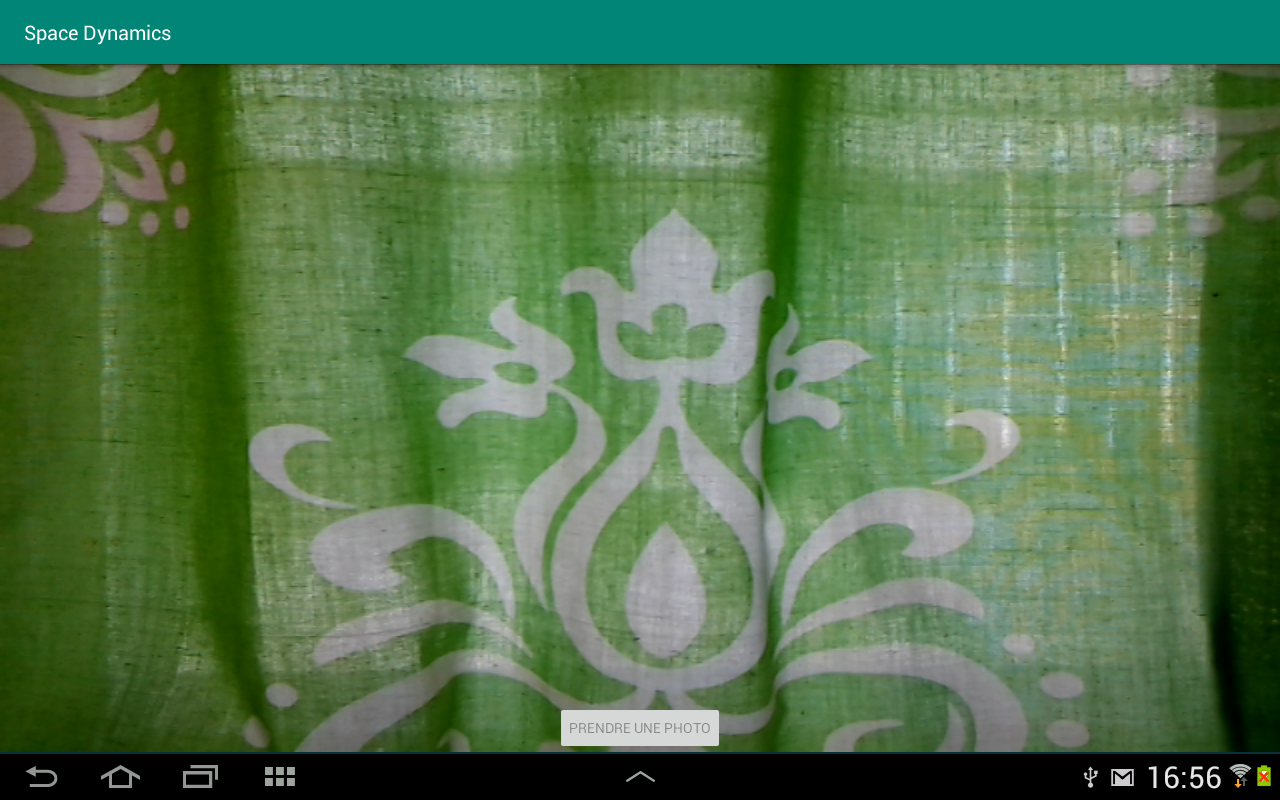
\includegraphics[scale=0.25]{CameraActivity.png}
\end{center}
Le menu caméra propose de :
\begin{itemize}
\item prendre une photo via un bouton approprié
\item prévisualiser l’environnement pour obtenir une photo de qualité optimale
\end{itemize}

\subsection{Menu fin de partie}
\begin{center}
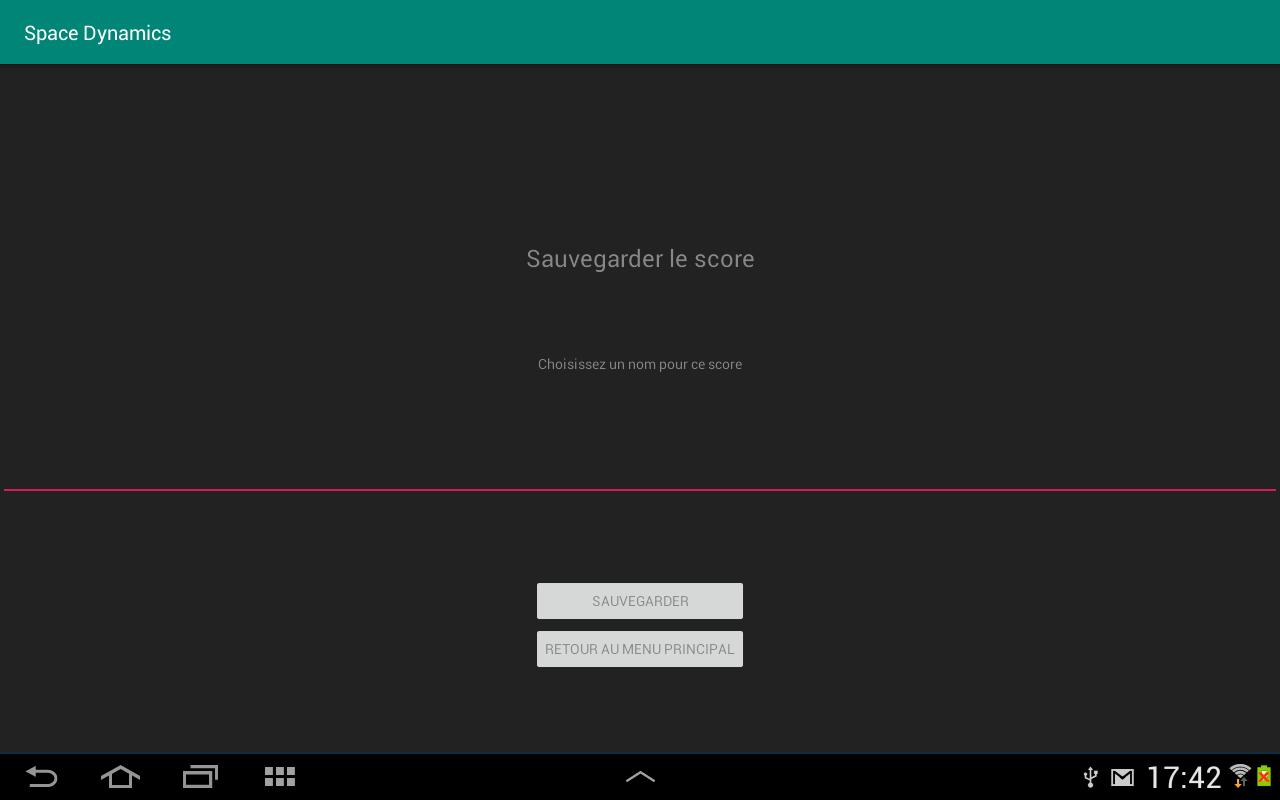
\includegraphics[scale=0.25]{EndGameActivity.png}
\end{center}
Le menu de fin de partie propose de :
\begin{itemize}
\item nommer le score
\item sauvegarder le score du joueur 
\item retourner au menu principal
\end{itemize}

\subsection{Menu chargement des sauvegardes}
\begin{center}
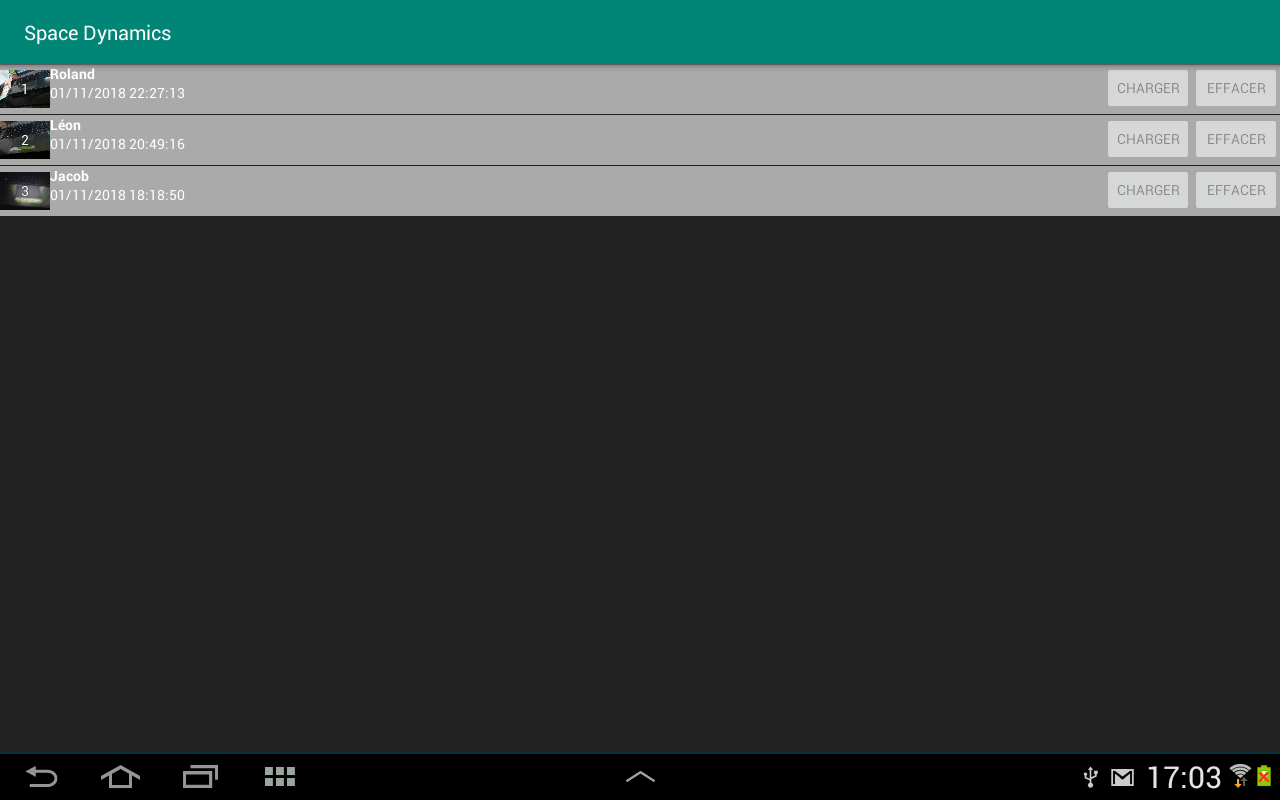
\includegraphics[scale=0.25]{LoadGameActivity.png}
\end{center}
Le menu de chargement des sauvegardes propose de :
\begin{itemize}
\item consulter les parties sauvegardées ainsi que les photos associées à chaque sauvegarde
\item charger une partie sauvegardée via le bouton charger
\item effacer une partie sauvegardée via le bouton effacer
\end{itemize}
Les sauvegardes sont présentées dans une liste classée par ordre chronologique décroissant.

\subsection{Menu affichage des scores}
\begin{center}
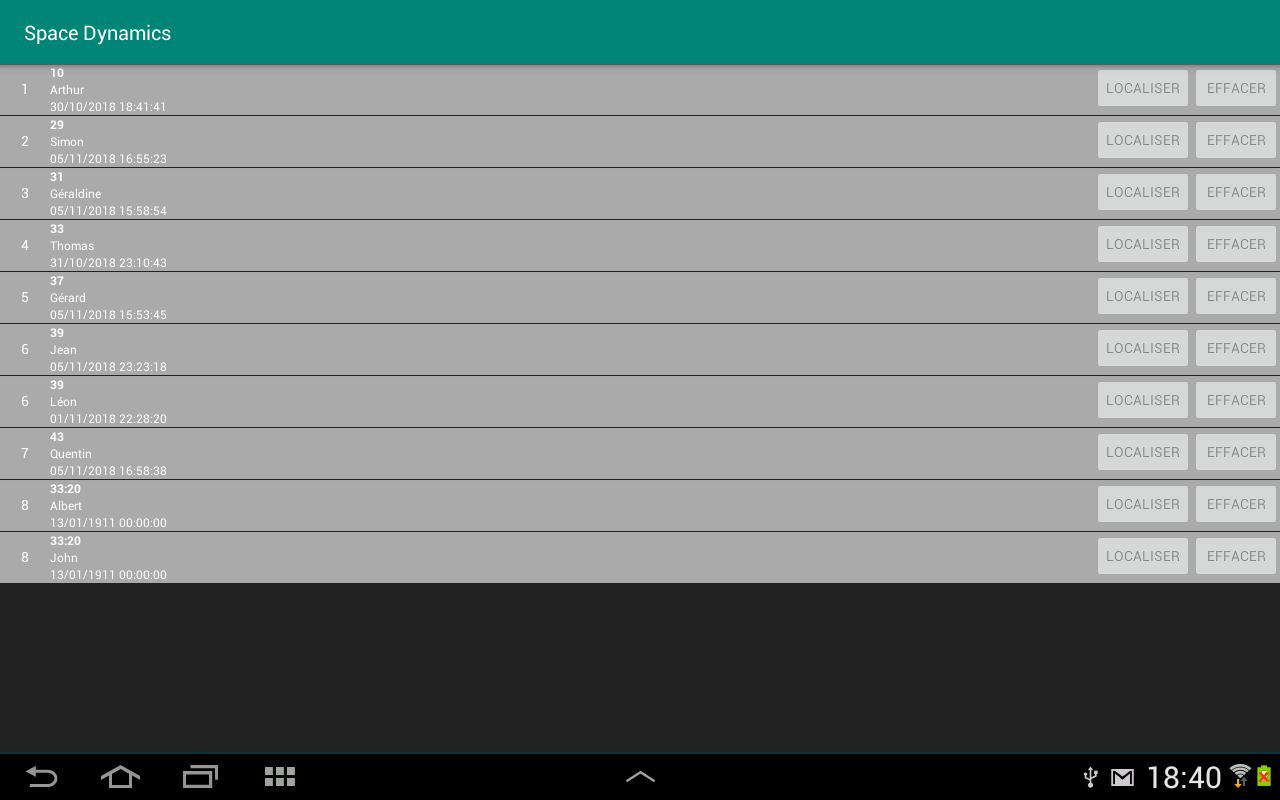
\includegraphics[scale=0.25]{ShowScoresActivity.png}
\end{center}
Le menu d'affichage des scores propose de :
\begin{itemize}
\item afficher les scores enregistrés
\item localiser un score sur une carte via le bouton localiser
\item effacer un score via le bouton effacer
\end{itemize}
Les scores sont présentés dans une liste classée d'abord par ordre croissant des scores puis par ordre alphabétique sur les noms associés aux scores.

\subsection{Menu localisation}
\begin{center}
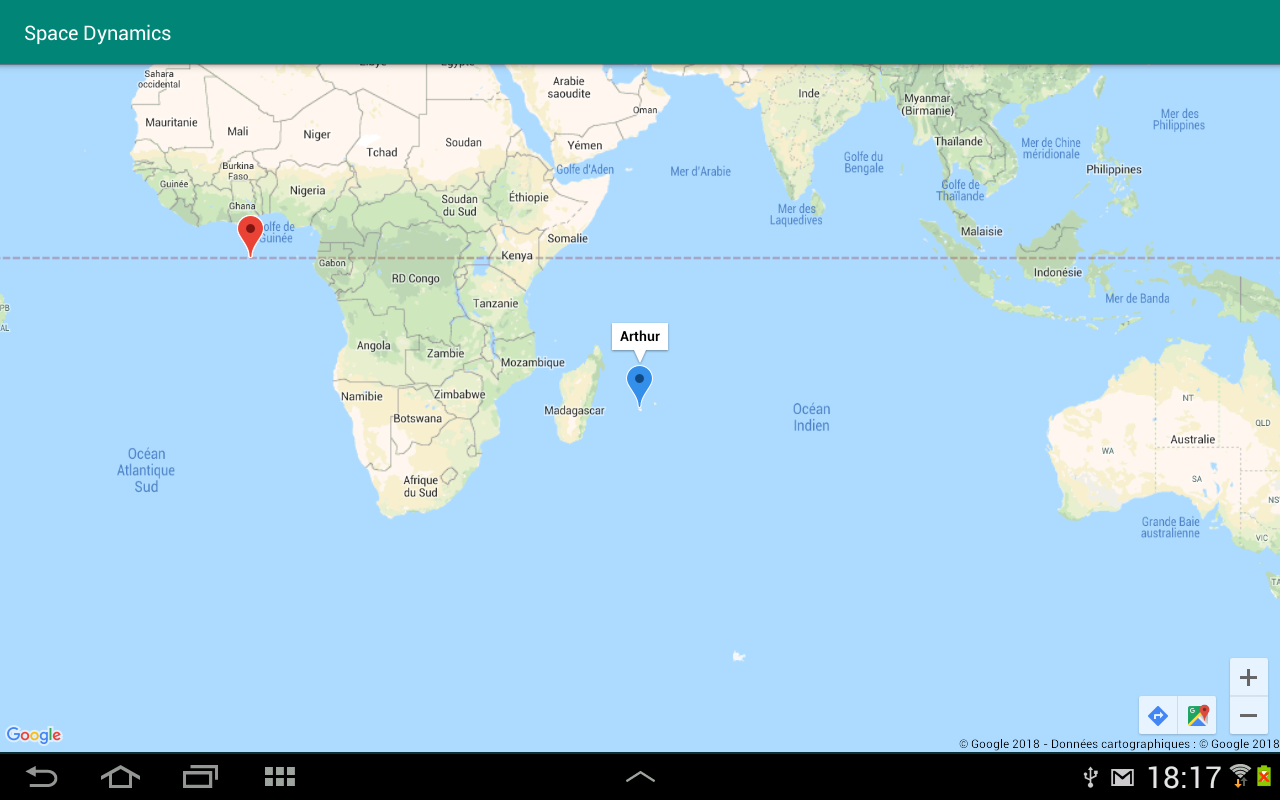
\includegraphics[scale=0.25]{MapsActivity.png}
\end{center}
Le menu localisation propose de :
\begin{itemize}
\item situer en bleu le score d’un joueur sélectionné depuis le menu d’affichage des scores
\item situer en rouge tous les autres scores 
\end{itemize}



\section{Architecture du code}

\subsection{Android}

\subsubsection{Diagramme de classes}
\begin{center}
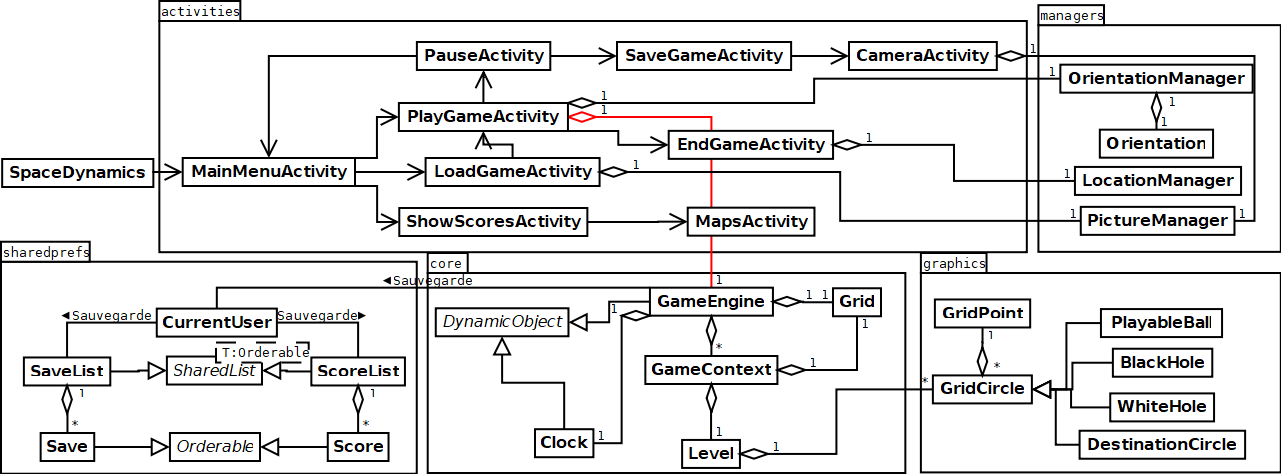
\includegraphics[scale=0.25]{Diagram.png}
\end{center}
Le diagramme de classe met en évidence 5 packages que nous allons détailler. Il ne permet pas de représenter tous les fichiers du projet mais donne une vision d'ensemble des interactions entre les classes, nous détaillerons également ces fichiers non représentables.

\paragraph{SpaceDynamics}
Une classe représentant l'application servant essentiellement à partager le contexte d’application à toutes les autres classes via un attribut statique.

\paragraph{Tools}
Le fichier Tools.kt contient un ensemble d’outils génériques destinés à toutes les classes.

\subsubsection{Les activités}

\paragraph{MainMenuActivity}
L'activité qui gère le menu principal est constituée de boutons permettant de :
\begin{itemize}
\item démarrer une nouvelle partie (via PlayGameActivity)
\item charger une partie existante (via LoadGameActivity)
\item consulter la liste des scores (via ShowScoresActivity)
\item mettre fin à l'application
\end{itemize}

\paragraph{PlayGameActivity}
L’activité qui gère l’interface de jeu via la vue GameBoardView traite la totalité des mécanismes de jeu en utilisant :
\begin{itemize}
\item GestureDetectorCompat pour le double tap déclenchant le menu pause (via PauseActivity)
\item OrientationManager pour les changements d’inclinaison
\item MediaPlayer pour la musique d’arrière-plan
\item GameEngine pour la supervision des évènements de jeu
\end{itemize}

\paragraph{PauseActivity}
L’activité qui gère le menu pause est constituée de boutons permettant de :
\begin{itemize}
\item reprendre la partie suspendue (via l’arrêt de l’activité courante)
\item sauvegarder la partie suspendue (via SaveGameActivity)
\item retourner au menu principal (via MainMenuActivity et l’arrêt des activités précédentes)
\end{itemize}

\paragraph{SaveGameActivity}
L’activité qui gère la sauvegarde de la partie est constituée d’un champ de texte permettant de modifier le nom de la partie courante et de boutons permettant de :
\begin{itemize}
\item prendre une photo (via CameraActivity)
\item sauvegarder la partie
\item retourner au menu pause (via l’arrêt de l’activité courante)
\end{itemize}

\paragraph{CameraActivity}
L’activité qui gère la prise de photo est constituée d’une surface de prévisualisation et d’un bouton permettant de prendre une photo. Une fois la photographie prise, celle-ci est enregistrée et référencée par PictureManager puis l’activité se termine.

\paragraph{EndGameActivity}
L’activité qui gère la sauvegarde des scores une fois la partie terminée est constituée d’un champ de texte permettant de nommer le score et de boutons permettant de :
\begin{itemize}
\item sauvegarder le score
\item retourner au menu principal (via MainMenuActivity et l’arrêt des activités précédentes)
\end{itemize}
Pour la sauvegarde du score, l'activité récupère la position de l’utilisateur via GeolocationManager.

\paragraph{LoadGameActivity}
L’activité qui gère le chargement des sauvegardes va les présenter dans une liste, classée par ordre chronologique décroissant puis alphabétique sur les noms, qu'elle récupère à partir du singleton SaveList. Chacune des entrées est constituée d’un rang (à gauche), surplombant éventuellement une photographie, et de deux boutons à droite, l’un pour charger la partie (via PlayGameActivity), l’autre pour la supprimer.

\paragraph{ShowScoresActivity}
L’activité qui gère l’affichage des scores va les présenter dans une liste, classée par ordre croissant selon les scores puis par ordre alphabétique sur les noms, qu'elle récupère à partir du singleton ScoreList. Chacune des entrées est constituée d’un rang (à gauche) et de deux boutons à droite, l’un pour localiser le score (via MapsActivity), l’autre pour le supprimer.

\paragraph{MapsActivity}
L’activité qui gère la représentation de la position géographique des scores sur une carte va représenter en bleu le score choisi depuis le menu d’affichage des scores et tous les autres scores en rouge. Les marqueurs sont nommés d'après les noms associés aux scores et la caméra est centrée sur le score sélectionné préalablement.

\subsubsection{Les éléments graphiques}

\paragraph{GridCircle}
Un cercle de grille est défini par une position dans une grille, une couleur et un rayon. Il définit une entité abstraite pour un objet circulaire qui peut être dessiné dans une grille.

\paragraph{PlayableBall}
Une balle jouable est un cercle de grille conçu pour être déplacé, il a une position initiale, un état de verrouillage et un état d’achèvement. Ces paramètres permettent respectivement de réinitialiser sa position, de la verrouiller pour effectuer des animations, et valider l’atteinte de sa destination.

\paragraph{DestinationCircle}
Un cercle de destination est un cercle de grille correspondant à la destination d’une balle jouable, il va servir à capturer les balles de la même couleur que lui.

\paragraph{BlackHole}
Un trou noir est un cercle de grille qui réinitialise la position des balles jouables.

\paragraph{WhiteHole}
Un trou blanc est un cercle de grille qui repousse les balles jouables.

\subsubsection{Le coeur}

\paragraph{DynamicObject}
Un objet dynamique est une entité abstraite assurant l’autonomie des objets instanciés par ses classes filles via un thread dédié et un mécanisme du contrôle du cycle de vie.

\paragraph{Clock}
Une horloge est un objet dynamique dessinable décrivant l'écoulement du temps.

\paragraph{GameEngine}
Un moteur de jeu est un objet dynamique supervisant l’ensemble d'une partie en définissant la grille, l’horloge et en déclenchant le passage des niveaux.

\paragraph{GameContext}
Un contexte de jeu est une sorte de moteur physique dans la mesure où il traite les mouvements et différencie 3 types de collisions (toucher, chute et capture). Le contexte ne dure que le temps d'un niveau, il change à chaque passage au niveau suivant.

\paragraph{Grid}
Une grille est une abstraction mathématique pour les dessins sur l’écran. Les dimensions théoriques de celle-ci sont constantes tandis que ses dimensions réelles s’ajustent automatiquement par rapport à la taille de l’écran. Cette grille peut être matérialisée pour la conception de niveaux de jeu mais cette possibilité est inactive au cours d'une partie.

\paragraph{Levels}
Le fichier Levels.kt contient la structure utilisée pour définir un niveau de jeu ainsi que la liste complète de ceux-ci. Cette liste est un tableau accessible exclusivement depuis le moteur de jeu via les extensions de propriétés que permet Kotlin.

\paragraph{DataClasses}
Le fichier DataClasses.kt contient un ensemble de classes distinctes mais similaires par le fait qu’elles ne définissent aucune méthode explicitement. Ainsi, il est préférable de les regrouper dans le même fichier plutôt que d’en avoir plusieurs dispersés un peu partout. Dans ce fichier, on trouve :
\begin{itemize}
\item Orientation : une structure regroupant les propriétés azimut, pitch et roll
\item GridPoint : une structure regroupant les coordonnées bidimensionelles d'un point d’une grille
\item Orderable : une classe facilitant le classement des instances de ses classes filles
\item Save : une structure définissant les éléments à préserver dans une sauvegarde
\item Score : une structure définissant les éléments à préserver dans un score
\end{itemize}

\subsubsection{Les gestionnaires}

\paragraph{IntentManager}
Le fichier IntentManager.kt facile la navigation et le passage de paramètres entre activités en définissant pour chacune d'elles des extensions de fonctions Kotlin au format :
\begin{verbatim}
fun X.toY(arg1, arg2, …)
\end{verbatim}
Exemple :
\begin{verbatim}
this@ShowScoresActivity.toMapsActivity(selectedScore)
\end{verbatim}

\paragraph{GeolocationManager}
Le gestionnaire de géolocalisation va encapsuler les mécanismes de géolocalisation de l'API pour renvoyer, via un attribut statique, la localisation actuelle de l'utilisateur.

\paragraph{OrientationManager}
Le gestionnaire d'orientation va encapsuler les mécanismes d'orientation de l'API pour renvoyer, via un attribut statique,
l'orientation courante de l'appareil mobile.

\paragraph{PictureManager}
Le gestionnaire d’images est un singleton qui va gérer l’association entre les sauvegardes et leur fichier image. Lors de son instanciation, il va supprimer tout fichier du dossier d’images non référencé par une sauvegarde ou ayant un identificateur non conforme. Il va permettre de récupérer un fichier image à partir de son identificateur depuis le dossier qu'il traite et il s’assurera de renvoyer l’identifiant le plus pertinent pour l'ajout de futures images au dossier.

\subsubsection{Les préférences partagées}

\paragraph{CurrentUser}
L'utilisateur courant est un singleton détenant toutes les informations concernant la partie en cours. Il garantit notamment l’accès et la persistance de ces données entre les activités via des attributs encapsulant les préférences partagées.

\paragraph{SharedList}
Une liste partagée est une liste abstraite d'éléments ordonnables encapsulant les préférences partagées. Bien qu'elle ne définisse que peu de méthodes publiques, elle peut être manipulée aussi simplement que les collections Java et Kotlin. Toutefois, afin de préserver la validité d'une instance, il convient de respecter un certain nombre de précautions :
\begin{itemize}
\item les préférences partagées encapsulées par l'instance ne devront plus être utilisées ailleurs
\item les listes filles devront être des singletons
\item les listes filles devront implémenter correctement les méthodes de mises en forme des données
\end{itemize}

\paragraph{SaveList}
La liste des sauvegardes est une liste partagée spécialisée pour les sauvegardes.

\paragraph{ScoreList}
La liste des scores est une liste partagée spécialisée pour les scores.


\subsection{iOS}
Implémentation abandonnée



\section{Quelques points délicats/intéressants}

\subsection{Les collisions}
\begin{center}
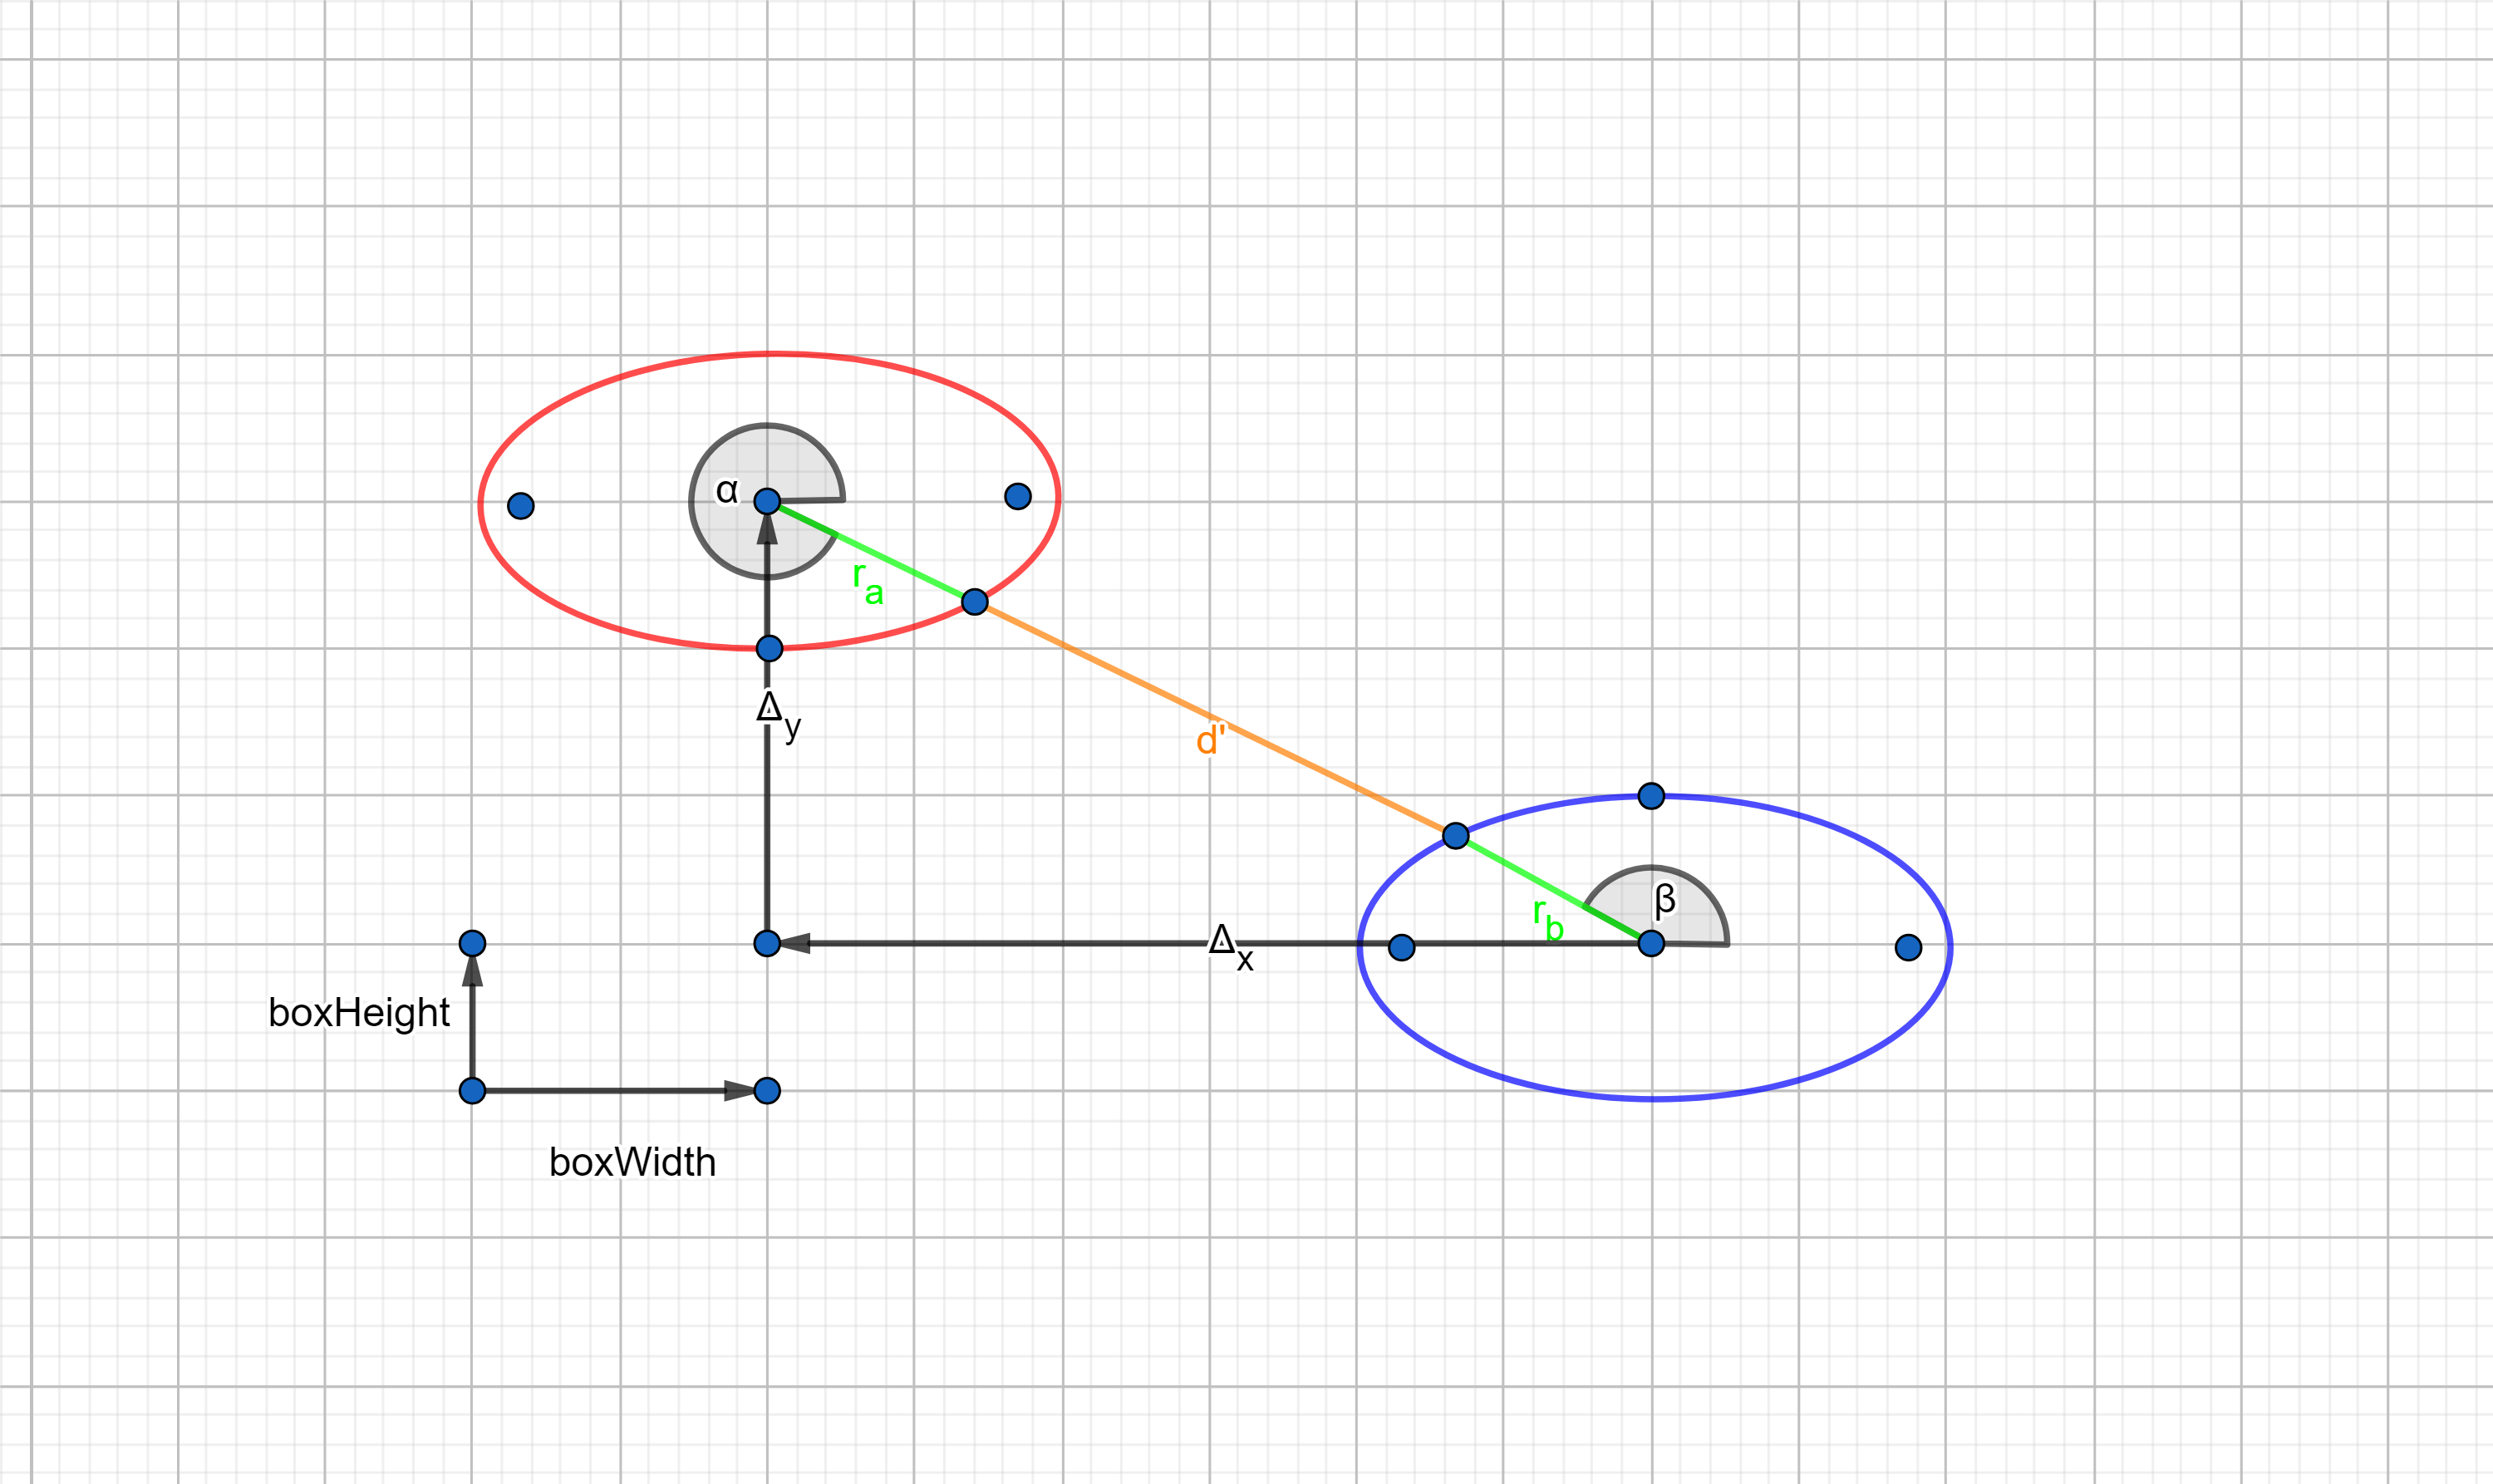
\includegraphics[scale=0.25]{Collision.png}
\end{center}
En apparence, la collision entre deux \textit{ellipses}~\cite{ellipseDoc} n'est pas très différente de celle entre deux cercles. Cependant, en pratique, il faut connaitre le rayon des ellipses pour détecter leur collision et, puisque celui-ci dépend de l'angle selon lequel on le calcule, la formule est beaucoup plus lourde.

\subsection{La géolocalisation}
La récupération de la position géographique s’effectue via une fonction de rappel. Ainsi, il est possible qu'au moment où en ait besoin cette position ne se soit pas encore valide car la fonction n'aura pas encore été appelée. Cette difficulté peut être contournée par un stockage temporaire de la valeur que l'on va récupérer tardivement mais ça reste un procédé hasardeux.

\subsection{Kotlin}
Le langage \textit{Kotlin}~\cite{kotlinDoc} a de très nombreux avantages par rapport à Java. Il est plus permissif, moins redondant, plus fiable et il dispose de nombreuses fonctionnalités supplémentaires. Détaillons quelques-unes de ses spécificités par rapport à Java :

\paragraph{Les extensions}
Kotlin propose l'\textit{extension}~\cite{extensionDoc} de propriétés et de fonctions afin d'enrichir les classes existantes.
Il faut toutefois faire attention aux conflits de noms car la documentation indique que, dans ce cas, une extension de propriété serait ignorée alors qu'une extension de fonction serait prise en compte. L'exemple d'extension de fonction suivant provient du fichier Tools.kt :
\begin{verbatim}
fun Any.Logd(msg: String) = Log.d(this::class.java.simpleName, msg)
\end{verbatim}
Cette extension visant la classe Any (racine de la hiérarchie de classe de Kotlin) va ajouter à toutes les classes une méthode d'instance qui s'appelera Logd et qui affichera le nom de la classe et un message. Il est intéressant de remarquer que si on tente d'appeler cette méthode comme s'il s'agissait d'une méthode statique, le nom affiché va correspondre à celui de l'objet compagnon puisque Kotlin traite les méthodes statiques comme des méthodes d'instances de cet objet compagnon.

\paragraph{Les singletons}
Kotlin définit la notion de \textit{singleton}~\cite{singletonDoc} via le mot clé object, il est tentant de vouloir l’utiliser autant que possible mais mal utilisé il peut causer des dysfonctionnements difficiles à identifier. De plus, Kotlin interdit le passage de paramètres aux constructeurs de ces singletons donc, s’ils sont indispensables, il faut soit se débrouiller pour ne pas avoir à passer de paramètres, soit utiliser un singleton pattern plus classique avec une classe ordinaire, un constructeur privé et une méthode statique getInstance. 

\section*{Conclusion}
Ce projet a été particulièrement enrichissant. En particulier, la découverte de Kotlin au cours de l'implémentation a été assez plaisante puisqu'elle a permis une progression rapide. Bien que le projet ait été pensé pour être très simple, il est finalement beaucoup plus élaboré que prévu et ce n’est pas plus mal puisqu’il a nécessité un approfondissement plus poussé de notions avancées.

Le projet n’est qu’une version de démonstration et n’a pas la prétention d’être publiable mais s’il devait l’être il est certain qu’il irait vers une représentation de l’espace plus réaliste avec un véritable moteur physique, des spirales, des astéroïdes à la place des balles, des structures complexes telles que des systèmes solaires ou même d’autres objets célestes plus imprévisibles.

Il semble que la totalité des dysfonctionnements critiques constatés aient été corrigés mais aucun test vraiment poussé n’a réellement été effectué donc il est concevable qu’une situation non considérée finisse par survenir un jour ou l'autre.

%%% La bibliographie:
\bibliographystyle{plain}
\bibliography{biblio}

\end{document}
